\chapter{Napájecí systém vesty}
Napájecí systém vesty má za úkol poskytovat elektrický výkon v požadované kvalitě pro správnou funkci dalších obvodů ve vestě.

Primárním zdrojem energie vesty je lithium-polymerový akumulátor 2XLP7836140, s kapacitou 7600~\jedn{mAh}, který by měl zajistit dostatečnou časovou výdrž vesty. Akumulátor je vybaven ochrannými obvody proti přílišnému vybití pod hranici 2,75~\jedn{V} a přebití přes 4,30~\jedn{V}.

Úbytky napětí na modré, zelené LED 3,4~\jedn{V} a úbytky vznikající na spínacích prvcích při regulování jasu LED, dosahují větší hodnoty než je napětí akumulátoru, bylo tedy nutné navrhnout napájecí systém založený na zvyšujícím měniči napětí.

Dalším úkolem napájecího systému je zajistit nabíjení akumulátoru a sledování stavu akumulátoru.

\section{Zvyšující měnič}
\begin{figure}[H]
    \begin{center}
        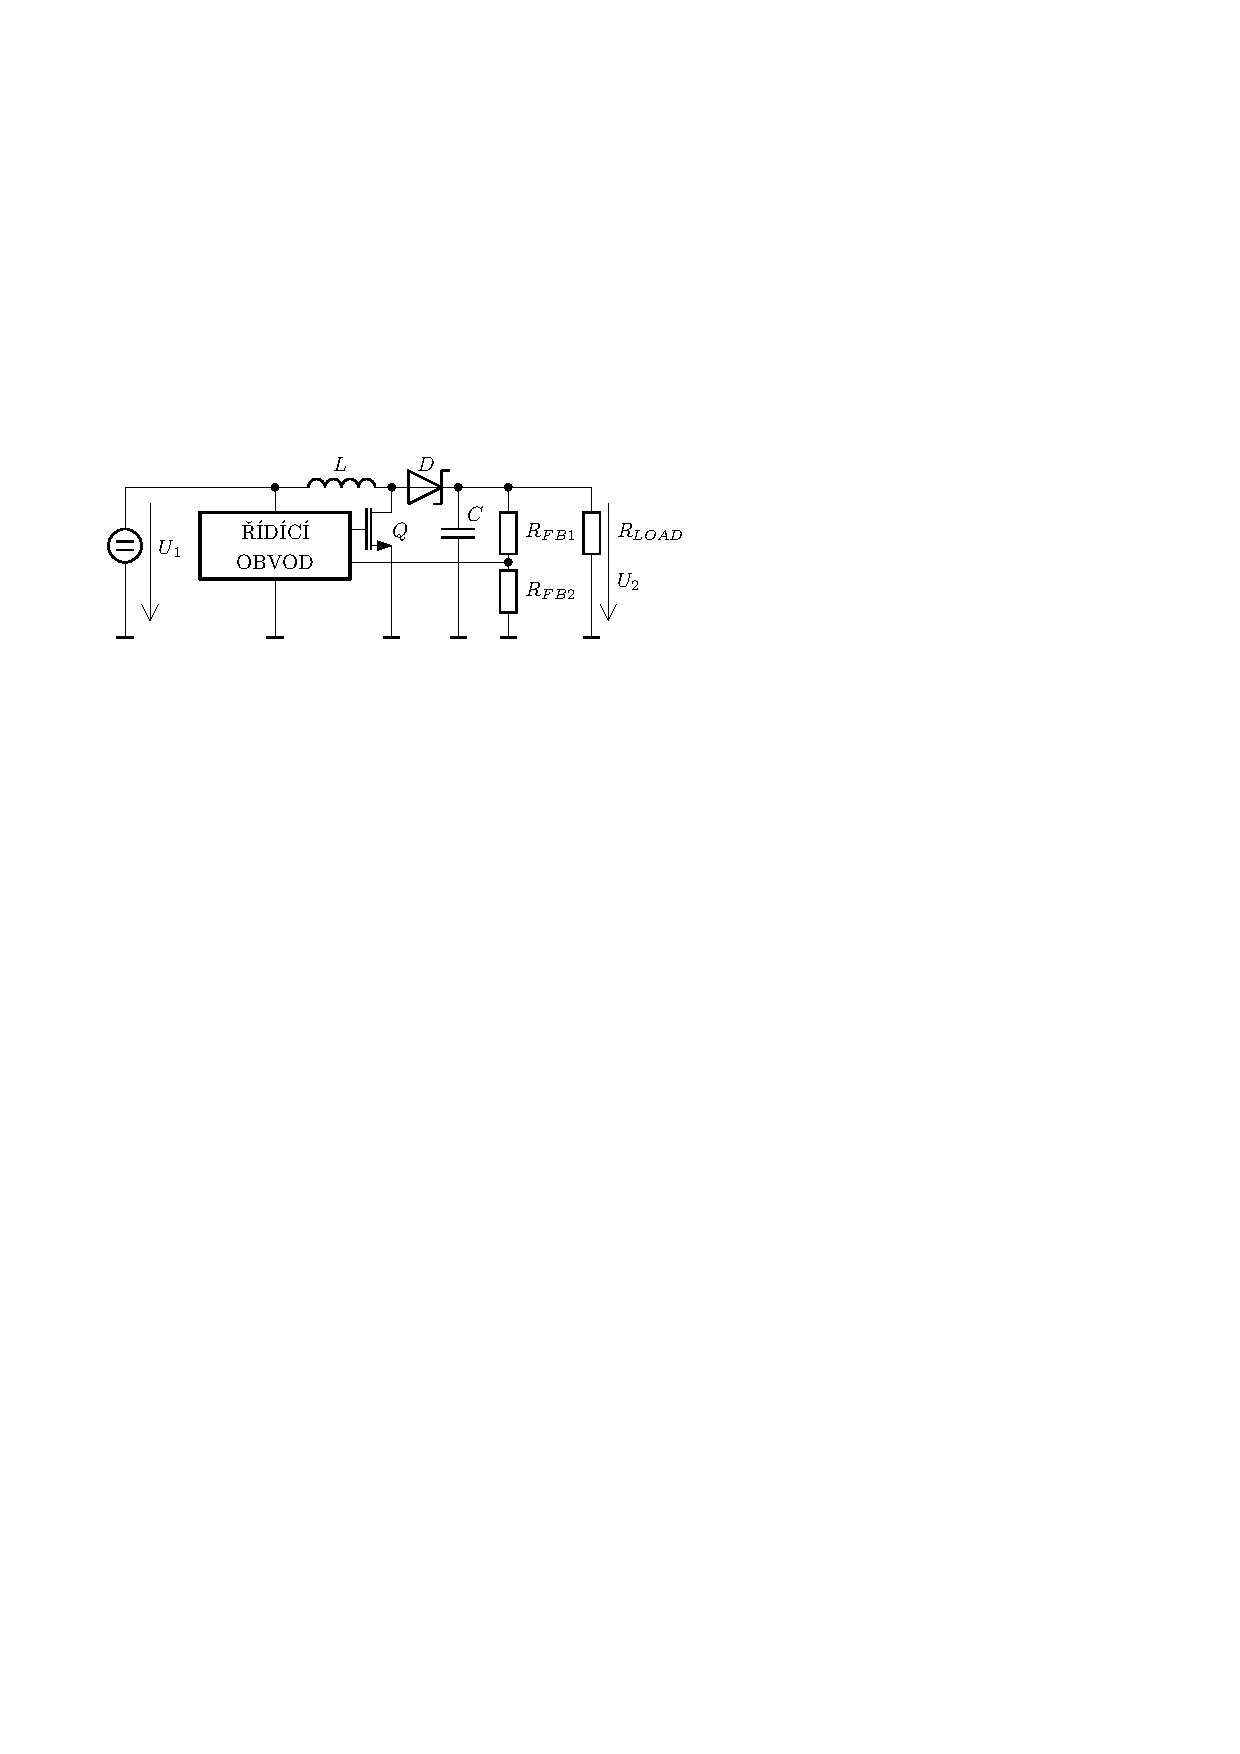
\includegraphics[width=\textwidth]{img/boost}
    \end{center}
    \caption{Blokové schéma zvyšujícího měniče}
\end{figure}
Zvyšující měnič, někdy také označovaný jako boost či step up, je elektrický obvod, patřící do kategorie spínaných měničů, které s vysokou účinností transformují vstupní napětí $U_1$ na vyšší napětí $U_2$. Účinnost spínaných měničů dosahuje až 99~\jedn{\%}, ztráty jsou způsobeny především přeměnou části transformované elektrické energie v teplo na spínacích prvcích a ohmickém odporu vinutí cívky. Účinnost se dá zvýšit použitím měniče, který místo diody používá tranzistor. Vstupní i výstupní napětí měniče jsou stejnosměrná.

Měnič obsahuje dva akumulační prvky $L$ a $C$, které slouží k uchování energie a dva prvky aktivní $Q$ a $D$, které plní funkci spínačů. Rezistor $R_{LOAD}$ představuje zátěž.

Ve chvíli sepnutí tranzistoru začne cívka akumulovat energii - v tento okamžik je dioda uzavřena, protože napětí na anodě má podprahovou hodnotu. Jakmile dojde k uzavření tranzistoru, otevře se dioda a začne přesouvat akumulovanou energii z cívky do kondenzátoru.

Odvození výstupního napětí zvyšujícího měniče pro ideální spínací prvky je následující:
\begin{eqnarray}
    i_L(t) &=& \dfrac{1}{L} \int u_L(t) \mathrm{d}t \Rightarrow u_L(t) = L \dfrac{\mathrm{d}i_L(t)}{\mathrm{d}t}
    \nonumber\\
    \dfrac{U_1 \cdot t_{ON}}{L} &=& \dfrac{(U_2 - U_1) t_{OFF}}{L} \Rightarrow U_1 \cdot t_{ON} = (U_2 - U_1) t_{OFF}
    \nonumber\\
    U_1 \cdot t_{ON} &=& U_2 \cdot t_{OFF} - U_1 \cdot t_{OFF} \Rightarrow U_1 \cdot T = U_2 \cdot t_{OFF}
    \nonumber\\
    U_2 &=& U_1 \dfrac{T}{t_{OFF}} = \underline{\underline{U_1 \dfrac{1}{1-s}}}
    \nonumber
\end{eqnarray}

Kde $t_{OFF}$ je čas, po který je tranzistor sepnut, $t_{OFF}$ čas po který je tranzistor rozepnut, $T$ je perioda spínání a $s$ střída spínání.

Ze vztahu lze vyvodit, že platí $U_2 \geq U_1$. Při použití reálných součástek tato rovnost neplatí, jestliže je tranzistor trvale rozepnut, je napětí $U_2$ menší o úbytek na diodě a cívce. Dále ze vztahu vyplývá, že velikost výstupního napětí je závislá pouze na velikosti vstupního napětí a střídě spínání.

Řídící obvod se snaží udržovat konstantní výstupní napětí pomocí regulování střídy. Výstupní napětí je monitorováno díky zpětné vazbě realizované napěťovým děličem. Poměr rezistorů $R_{FB1}$ a $R_{RB2}$ určuje výsledné výstupní napětí.

Pro realizaci zvyšujícího měniče byl vybrán integrovaný obvod firmy Linear Technology LTC1871.

\begin{figure}[H]
    \begin{center}
        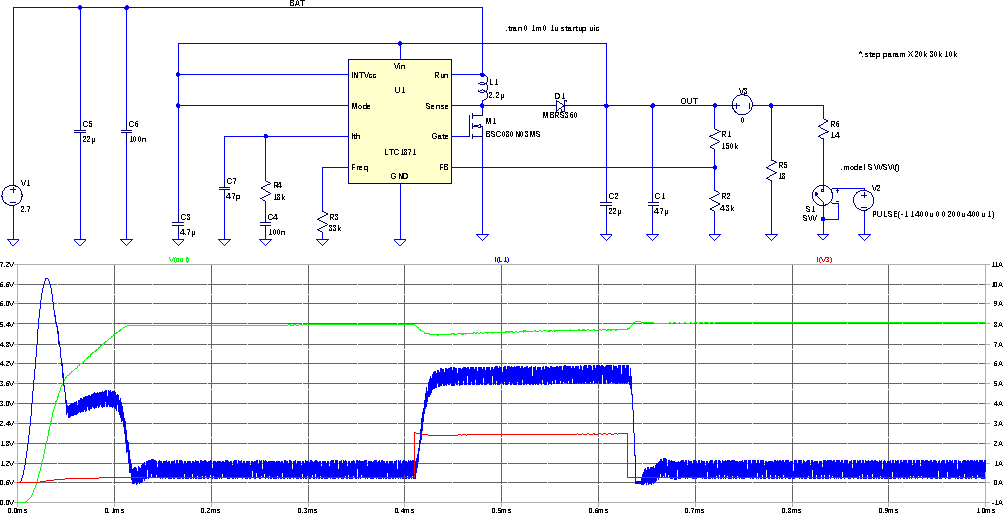
\includegraphics[width=\textwidth]{img/boost-sim}
    \end{center}
    \caption{Ověření funkce simulací zvyšujícího měniče v programu LTspice}
\end{figure}

\section{Nabíjecí obvod}
Nabíječka zajišťuje přesouvání energie z externího zdroje do akumulátoru - právě díky ní jsou akumulátory opakovatelně použitelné. Pro laser game arény je důležité, aby nabíječka byla schopná přes noc (12 hodin času) dobít akumulátory. Vezmeme-li v úvahu kapacitu akumulátoru a čas potřebný pro jeho nabití, zjistíme, že nabíječka musí být schopna nabíjet akumulátor minimálně proudem 633~\jedn{mA}, od čehož se musí odvíjet i výběr nabíjecího obvodu. Nakonec byl vybrán obvod BQ24192 od firmy Texas Instruments.

BQ24192 je určený k nabíjení lithium-iontových a lithium-polymerových akumulátorů. Je založen na snižujícím spínaném měniči, dokáže pracovat od napájecího napětí 3,9~\jedn{V} až 17~\jedn{V} a nabíjet proudem až 4,5~\jedn{A}. Je také schopen monitorovat teplotu článku pomocí termistoru. S okolím komunikuje prostřednictvím I2C sběrnice, která umožňuje nastavovat některé nabíjecí parametry.

\begin{figure}[H]
    \begin{center}
        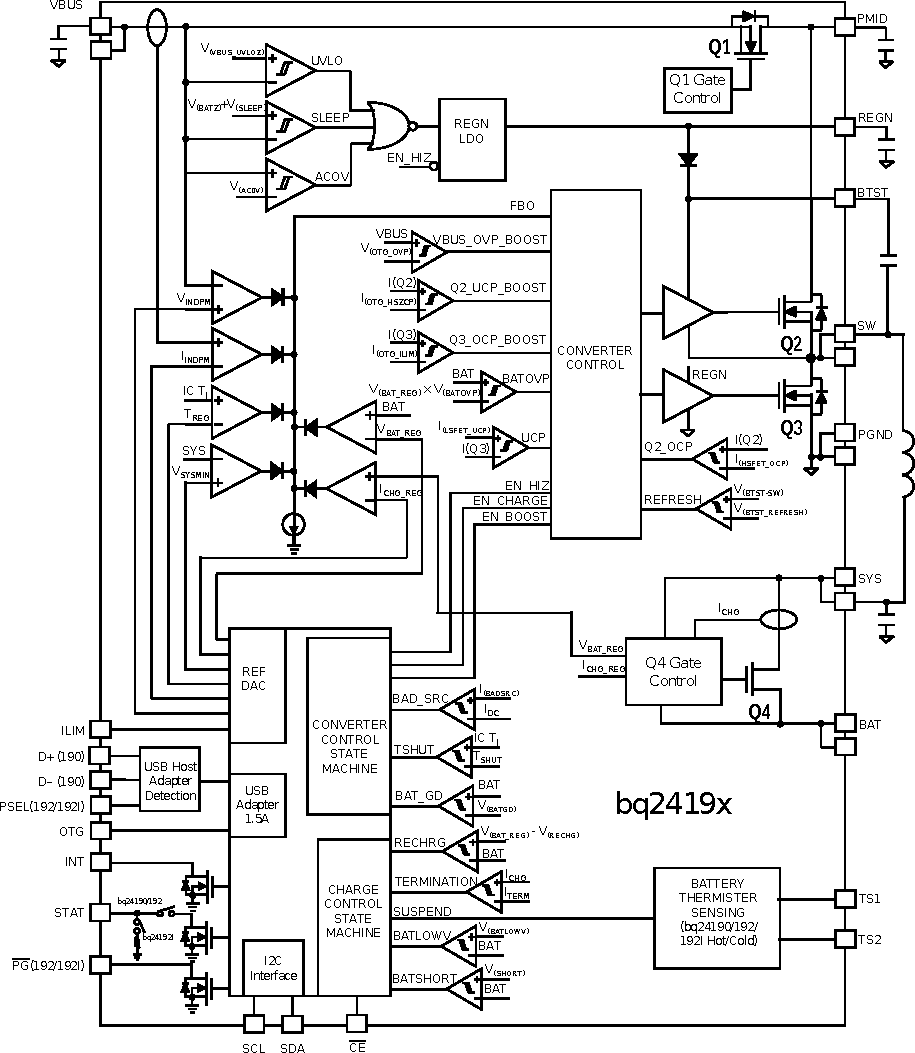
\includegraphics[width=\textwidth]{img/bq24192-block}
    \end{center}
    \caption{Nabíjecí obvod BQ24192, převzato z katalogového listu výrobce}
\end{figure}

Pinem PSEL se nastaví jestli je obvod napájen z USB (vysoká úroveň) a nebo adaptéru (nízká úroveň). \Overline{CE}~ povoluje nabíjení, \Overline{PG}~ signalizuje přítomnost napájecího napětí a STAT signalizuje stav nabíjení (vysoká úroveň signalizuje dokončení nabíjení). Velmi důležitým pinem je ILIM, který slouží k nastavení maximálního nabíjecího proudu pomocí rezistoru $R_{ILIM}$.

$$I_{IN MAX} = \dfrac{1~\jedn{V}}{R_{ILIM}} \cdot 530 = \dfrac{1}{180} \doteq \underline{\underline{3~\jedn{A}}}$$ \nonumber

\section{Monitorování náboje}
Monitorování stavu nabití akumulátoru je důležité zejména pro obsluhu arény, aby nedošlo k nechtěnému vypnutí vesty při aktivní hře. Signalizovat stav akumulátoru lze například i prostým děličem napětí, v případě, kdy by postačovalo rozlišování pouze dvou stavů, jinak analogově digitálním převodníkem. Tyto metody ale mají nevýhodu, že výstupní napětí akumulátoru se může měnit v závislosti na odebíraném proudu a vnitřním odporu akumulátoru. Obsluha pak může být mystifikována z fluktuací napětí a a může nesprávně vyhodnotit reálný stav akumulátoru. Proto tyto metody byly zavrženy a stav je vyhodnocován z celkového náboje.

\begin{figure}[H]
    \begin{center}
        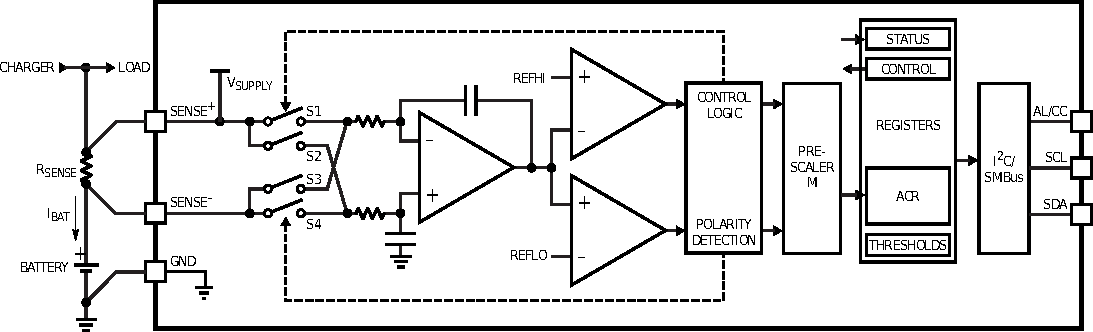
\includegraphics[width=\textwidth]{img/LTC2941-block}
    \end{center}
    \caption{Blokové schéma obvodu LTC2941, převzato z katalogového listu výrobce}
\end{figure}
Použil jsem integrovaný obvod LTC2941 firmy Linear Technology. Tento obvod je stále připojený k akumulátoru přes snímací rezistor malé hodnoty, ze kterého v klidu odebírá proud pod $100~\jedn{\mu A}$.

Obvod v pravidelných časových intervalech měří napětí na snímacím rezistoru a z jeho polarity určuje, jestli je akumulátor nabíjen či vybíjen, a z hodnoty napětí a známého času měření dopočítává náboj.

Obvod je vybaven I2C sběrnicí, takže je velmi snadné z něj vyčítat informace o náboji v systému.

\section{Topologie napájecího systému}
\begin{figure}[H]
    \begin{center}
        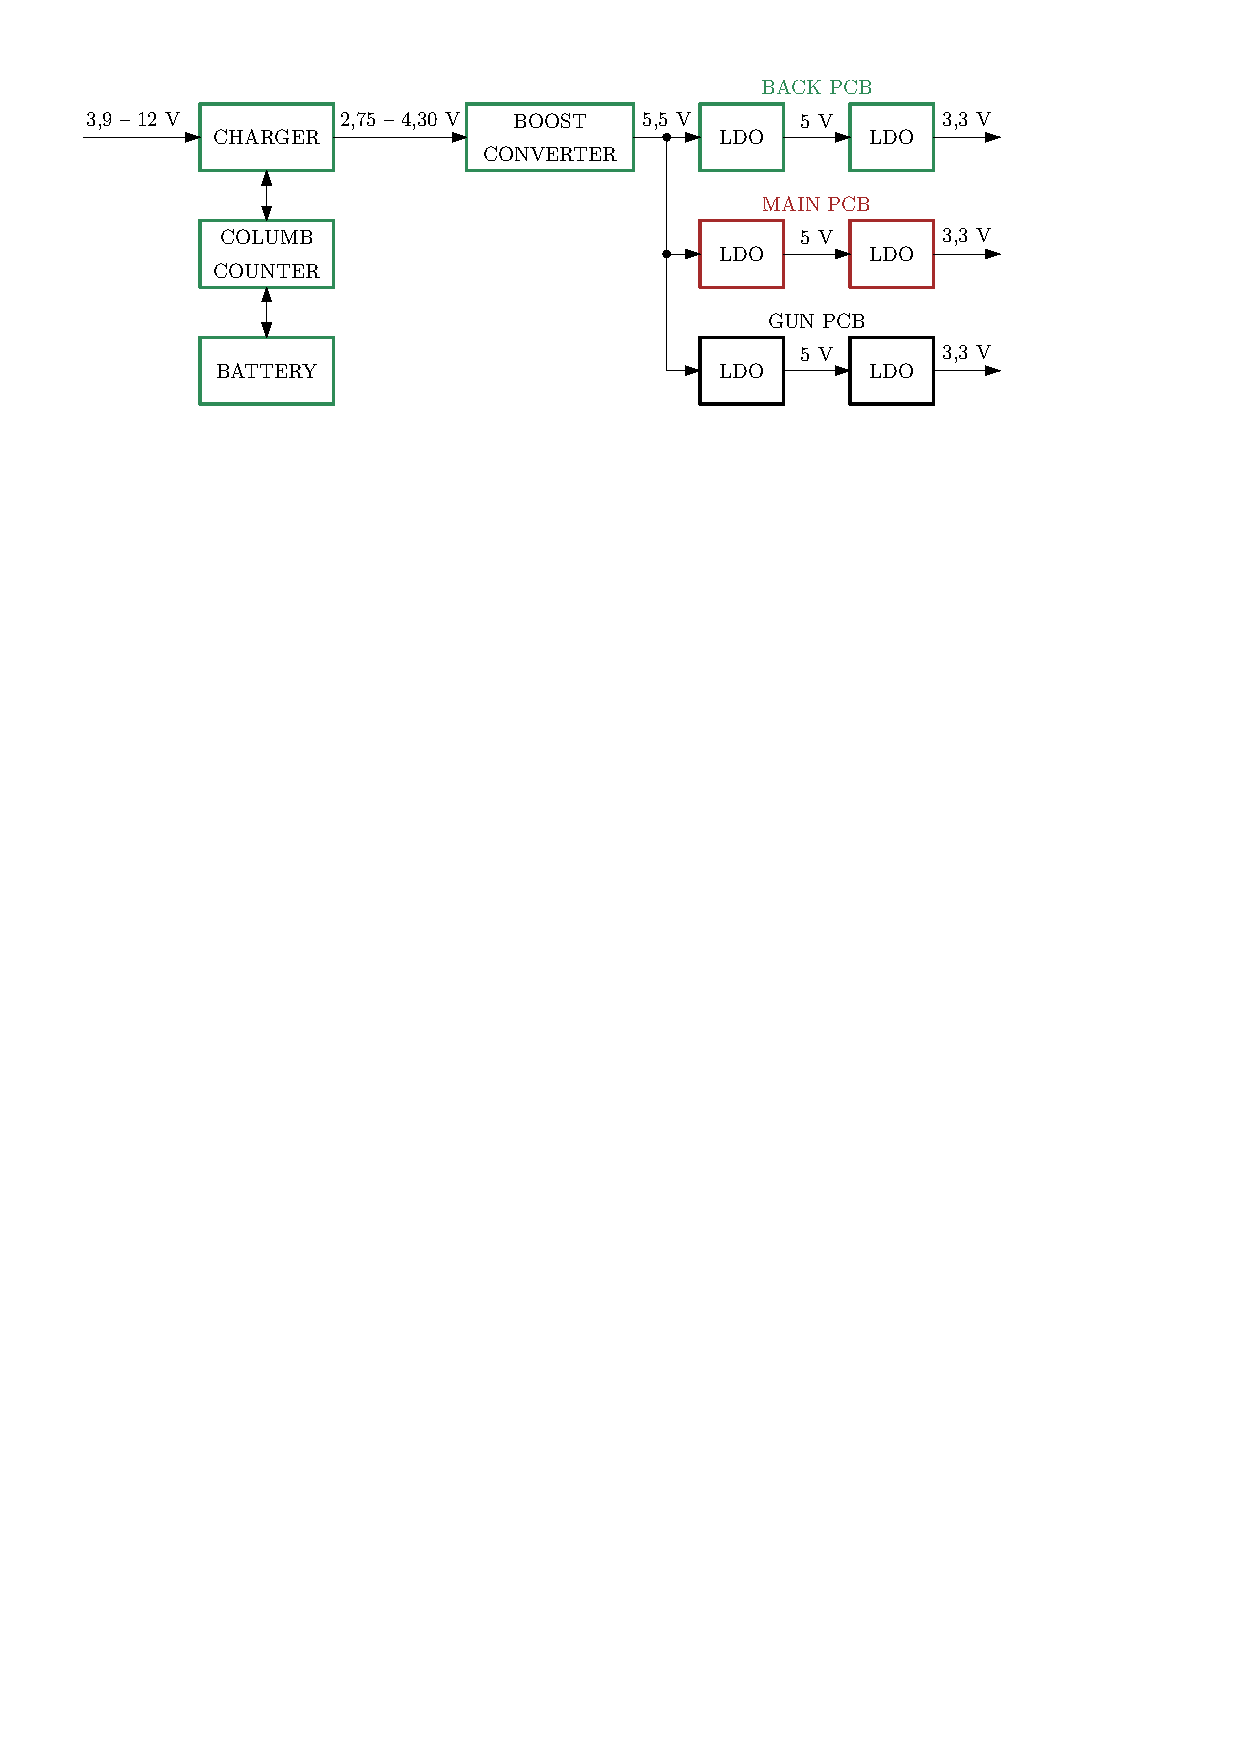
\includegraphics[width=\textwidth]{img/power-system}
    \end{center}
    \caption{Blokové schéma napájecího systému}
\end{figure}

Většina bloků napájecího systému se nachází na plošném spoji (PCB) pojmenovaném back, který je umístěn na zádech hráče. Ten obstarává monitorování náboje, nabíjení akumulátoru a zvyšování napětí akumulátoru. Do všech částí vesty je přiváděno napětí 5,5~\jedn{V}, které je na výstupu zvyšujícího měniče. Napětí je dále snižováno pomocí nízko-úbytkových stabilizátorů (LDO).
